\documentclass[11pt]{article}
\usepackage{../madar}
\newcommand{\madarissue}{العدد ١ · الجمعة ٢٠ نوفمبر ٢٠٢٦م}
\newcommand{\madarsite}{https://waleedasm19.github.io/artovia-site/}
\begin{document}

% ===================== الغلاف =====================
\thispagestyle{empty}
\begin{tikzpicture}[remember picture,overlay]
 \node[inner sep=0] at (current page.center) {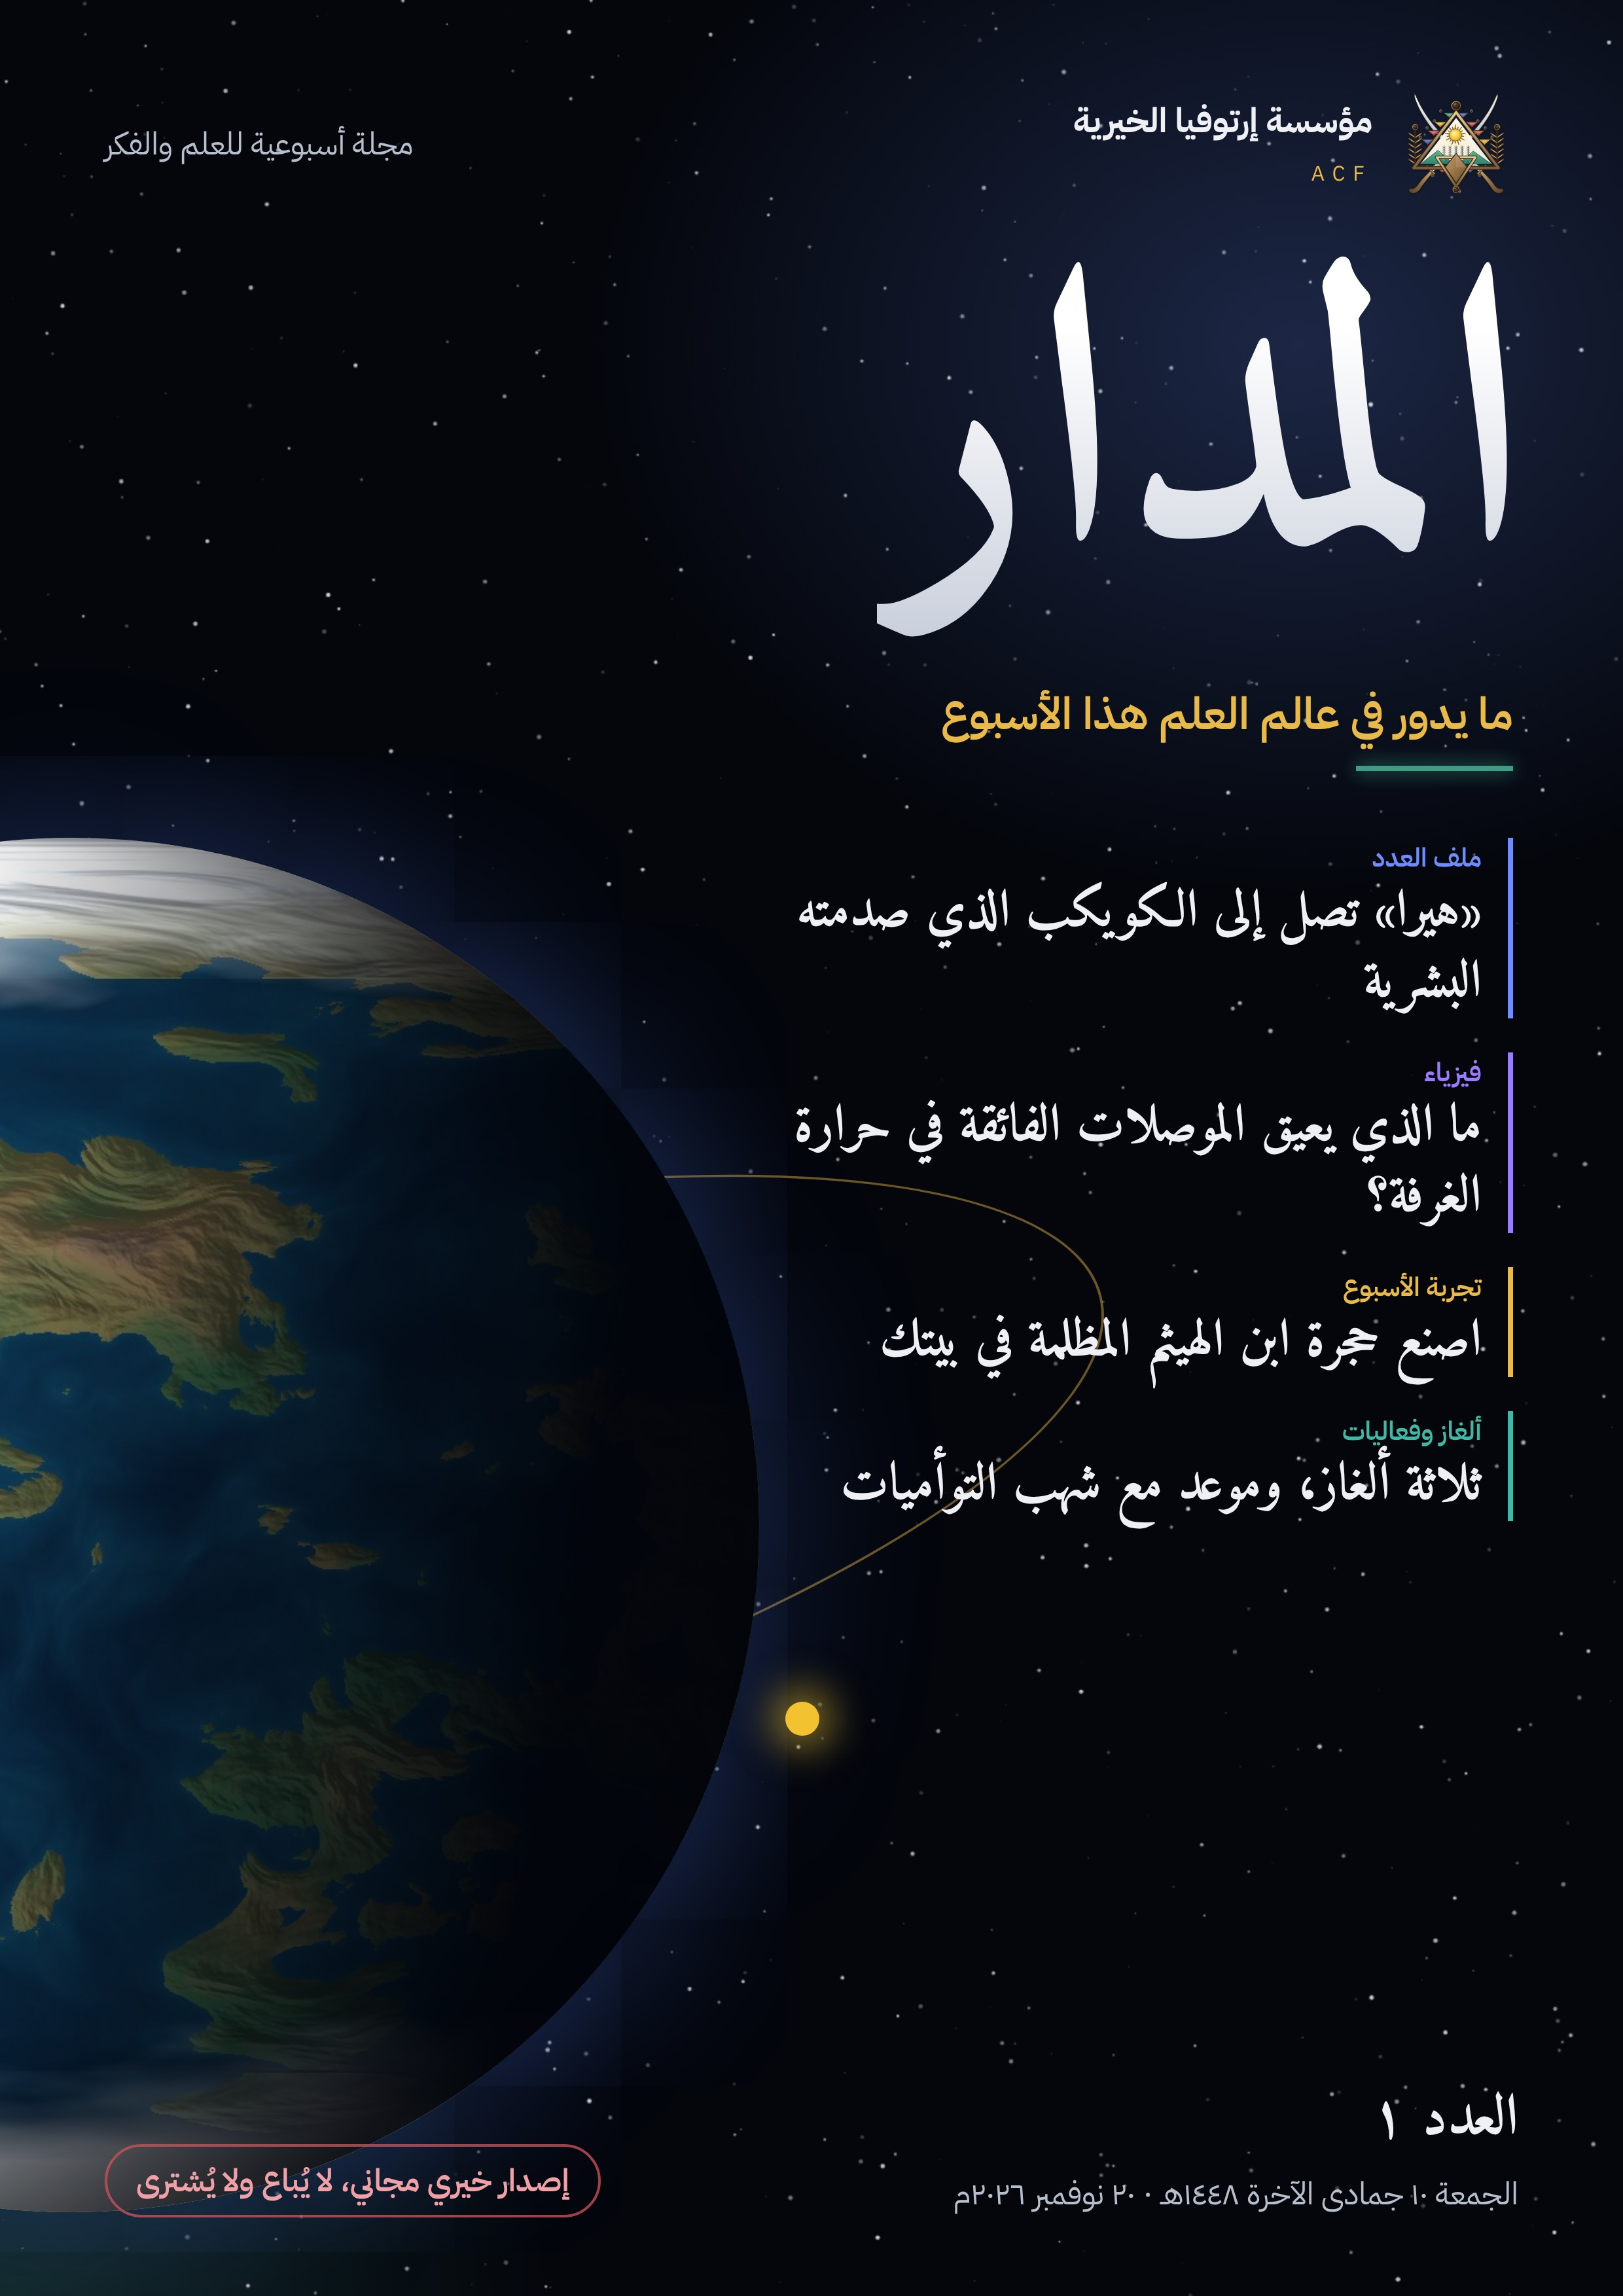
\includegraphics[width=\paperwidth,height=\paperheight]{cover.jpg}};
\end{tikzpicture}
\null\newpage

% ===================== الافتتاحية والفهرس =====================
\Section[gold]{كلمة العدد}
\Title{أهلًا بك في «المدار»}
\Deck{مجلة أسبوعية من مؤسسة إرتوفيا الخيرية، تصدر كل جمعة}

بين يديك العدد الأول من «المدار». اخترنا هذا الاسم لأن العلم يشبه الأجرام في مداراتها: يدور حول أسئلة كبرى لا تنتهي، وكلما اكتملت دورة بدأت دورة أوسع منها. في كل جمعة نجمع لك أهمّ ما دار في عالم العلم خلال الأسبوع، ونشرحه بعربية واضحة، ونذكر مصدر كل خبر مع رمز تمسحه بهاتفك لتقرأ الأصل بنفسك.

ولن نكتفي بالأخبار: في كل عدد ملفٌّ نتعمّق فيه، وتجربة تصنعها في بيتك، وفكرة نتأمّلها معًا، وألغاز تشحذ الذهن، ومواعيد لأحداث علمية تستحق أن ترفع لها رأسك إلى السماء.

هذه المجلة إصدار خيري مجاني، كسائر إصدارات المؤسسة. نرجو أن تجد فيها ما يوقظ فضولك، وأن تشاركها مع من يحب العلم.

\hfill{\sansfont\bfseries هيئة التحرير في مؤسسة إرتوفيا الخيرية}

\vspace{10pt}
\begin{feature}
{\sansfont\bfseries\color{gold}\large في هذا العدد}\par\vspace{4pt}
\begin{tabular}{@{}r@{\quad}l@{}}
{\sansfont\bfseries ٣} & أخبار الأسبوع: ثماني محطات من الفضاء إلى الطب\\
{\sansfont\bfseries ٥} & ملف العدد: «هيرا» تصل إلى الكويكب الذي صدمته البشرية\\
{\sansfont\bfseries ٦} & فكرة للتأمل: ابن الهيثم ومنهج الشك\\
{\sansfont\bfseries ٧} & تجربة الأسبوع: اصنع حجرة مظلمة في بيتك\\
{\sansfont\bfseries ٨} & فعاليات ومواعيد\\
{\sansfont\bfseries ٩} & ألغاز العدد\\
\end{tabular}
\end{feature}
\newpage

% ===================== أخبار الأسبوع =====================
\Section[blue]{أخبار الأسبوع}
\Title{ما دار في عالم العلم}
\Deck{ملخصات مختصرة، والتفاصيل في المصدر الأصلي: امسح الرمز}

\News[blue]{الفضاء}{مسبار «هيرا» يحلّق حول موقع اصطدام بشري بكويكب}{وصل مسبار وكالة الفضاء الأوروبية «هيرا» إلى الكويكب الصغير «ديمورفوس» ليدرس ما أحدثه اصطدام مهمة «دارت» التابعة لناسا به عام ٢٠٢٢م، وبدأ يلتقط صورًا للوجه المليء بالفوهات لرفيقه الأكبر «ديديموس». تفاصيل أوسع في ملف العدد.}{ScienceDaily / ESA}{https://www.sciencedaily.com/releases/2026/11/261115085545.htm}

\News[blue]{الفضاء}{«إقليدس» يرصد ٣١ كوازارًا من فجر الكون}{رصد تلسكوب «إقليدس» الأوروبي ٣١ كوازارًا قديمًا، وهي نوى مجرات شديدة السطوع يغذيها ثقب أسود هائل، من بينها جرمان حطّما الأرقام القياسية. ضوء هذه الأجرام انطلق والكون ما يزال في طفولته.}{ScienceDaily / ESA}{https://www.sciencedaily.com/releases/2026/11/261112230504.htm}

\News[violet]{الفيزياء}{ما الذي يعيق الموصلات الفائقة في حرارة الغرفة؟}{وجد باحثون أن الإلكترونات قادرة على تكوين أزواج مستقرة في درجات حرارة أعلى مما كان يُظن، ومع ذلك لا تظهر الموصلية الفائقة. معنى ذلك أن العائق أمام موصلات تعمل في حرارة الغرفة عائق آخر غير تكوّن الأزواج، وهو ما يعيد توجيه البحث في هذا الحلم القديم.}{ScienceDaily}{https://www.sciencedaily.com/releases/2026/11/261116023358.htm}

\News[violet]{الفيزياء}{التواء غامض في أقدم ضوء في الكون}{تلمح بعض القياسات إلى دوران طفيف في استقطاب إشعاع الخلفية الكونية، وهو أقدم ضوء يمكن رصده. إن ثبت فقد يشير إلى فيزياء جديدة، وقد طوّر فريق من جامعة كاليفورنيا في سان دييغو طريقة تساعد على استبعاد أن يكون خطأً في معايرة التلسكوبات.}{ScienceDaily}{https://www.sciencedaily.com/releases/2026/11/261116023348.htm}

\News[orange]{الكيمياء}{لماذا يتوهّج لهب الهيدروجين برتقاليًّا ثم يكاد يختفي؟}{لهب الهيدروجين النقي يكاد لا يُرى، وهذا خطر على السلامة. أوضحت دراسة جديدة أن آثارًا ضئيلة من الصوديوم العالق في الهواء هي ما يمنحه أحيانًا لونًا برتقاليًّا، وهي معرفة قد تساعد على تصميم أجهزة هيدروجينية أكثر أمانًا.}{ScienceDaily}{https://www.sciencedaily.com/releases/2026/11/261118065509.htm}

\News[teal]{الأرض والمناخ}{جروف الجليد في القارة القطبية الجنوبية: أسرع تراجعًا، وأقل كارثية}{شمل مسح جديد أكثر من ١٥ ألف جرف جليدي في القارة القطبية الجنوبية، وأشارت نتائجه إلى أنها قد تكون أقل عرضة للانهيار الكارثي المفاجئ مما كان يُخشى، مع أنها تتراجع بوتيرة أسرع من المتوقع.}{ScienceDaily}{https://www.sciencedaily.com/releases/2026/11/261117033925.htm}

\News[red]{الطب}{الشيخوخة تُضعف «نظام التنظيف» الليلي في الدماغ}{أظهر باحثون في معهد ماساتشوستس للتقنية أن تخلّص الدماغ من فضلاته أثناء النوم يضعف مع التقدّم في العمر، وربطوا ذلك بضعف موجات النوم العميق وتغيّر تدفق الدم في الدماغ.}{ScienceDaily / MIT}{https://www.sciencedaily.com/releases/2026/11/261114202137.htm}

\News[gold]{الهندسة}{روبوت يبني هيكلًا في المدار لأول مرة}{نجح روبوت طوّره باحثون في معهد كاليفورنيا للتقنية في بناء جزء من هيكل في الفضاء بشكل ذاتي، وهي خطوة أولى نحو تجميع تلسكوبات ومنشآت ضخمة في المدار بدل إطلاقها كاملة من الأرض.}{ScienceDaily / Caltech}{https://www.sciencedaily.com/releases/2026/11/261108233043.htm}
\newpage

% ===================== ملف العدد =====================
\Section[blue]{ملف العدد}
\Title{«هيرا» عند الكويكب الذي صدمته البشرية}
\Deck{ماذا نتعلّم من أول تجربة لتغيير مسار جرم سماوي؟}

في السادس والعشرين من سبتمبر ٢٠٢٢م اصطدمت مركبة ناسا «دارت» عمدًا بالكويكب الصغير «ديمورفوس»، وهو قمير يدور حول كويكب أكبر اسمه «ديديموس». لم يكن هذا الزوج يهدد الأرض، بل اختاره العلماء لأنه مختبر مثالي: يمكن قياس مدة دوران القمير حول رفيقه من الأرض بدقة، فإن تغيّرت بعد الاصطدام عرفنا أن الضربة غيّرت مساره.

وقد تغيّرت فعلًا: قصرت دورة «ديمورفوس» حول «ديديموس» بنحو نصف ساعة بحسب قياسات ناسا. كانت تلك أول مرة يغيّر فيها البشر حركة جرم سماوي عن قصد، وأول اختبار حقيقي لفكرة «الدفاع الكوكبي»: أن ندفع كويكبًا خطرًا دفعة صغيرة قبل سنوات من اقترابه، فيخطئ الأرض.

\begin{feature}
{\sansfont\bfseries\color{gold} لماذا نحتاج إلى «هيرا»؟}\par
أخبرتنا «دارت» أن المسار تغيّر، لكنها لم تخبرنا لماذا تغيّر بهذا القدر بالضبط. فقوة الدفع لا تأتي من المركبة وحدها، بل من الحطام الذي اندفع من سطح الكويكب في الاتجاه المعاكس كأنه محرك صاروخي. ومقدار هذا الحطام يعتمد على كتلة الكويكب وتماسك صخوره وشكل الحفرة. هذه هي الأسئلة التي جاءت «هيرا» لتجيب عنها من قرب.
\end{feature}

أُطلق المسبار الأوروبي في أكتوبر ٢٠٢٤م، ووصل الآن إلى الزوج الكويكبي. يحلّق «هيرا» حول موقع الاصطدام في مسارات مستطيلة الشكل، ويلتقط صورًا تكشف الوجه المليء بالفوهات لـ«ديديموس»، ويقيس كتلة «ديمورفوس» وشكله بعد الضربة. ويرافقه مسباران صغيران بحجم حقيبة اليد سيقتربان أكثر من السطح.

{\sansfont\bfseries\color{blue} ما الذي يعنيه ذلك لنا؟}\par
إن نجحت «هيرا» في تحويل تجربة «دارت» إلى أرقام دقيقة، صار لدى البشرية لأول مرة «وصفة» محسوبة: كم يلزم من الكتلة والسرعة لإزاحة كويكب من نوع معيّن بمقدار معيّن. إنها خطوة صغيرة في الفضاء، وكبيرة في حماية الأرض.

\vspace{6pt}
\begin{center}
\begin{tikzpicture}[scale=1]
 \fill[night,rounded corners=3mm] (-7.5,-2.2) rectangle (7.5,2.4);
 \foreach \x/\y in {-6.8/1.9,-5.2/-1.6,-3.6/2.0,-1.4/-1.9,0.8/2.1,2.9/-1.7,4.6/1.8,6.6/-1.2,6.9/2.1,-6.2/-0.6}{\fill[white,opacity=.7] (\x,\y) circle (0.03);}
 \shade[ball color=brown!60!gray] (2.2,0) circle (1.25);
 \draw[goldL,dashed,thick] (2.2,0) ellipse (3.4 and 1.1);
 \shade[ball color=gray!70] (-1.2,0.25) circle (0.32);
 \draw[red,very thick,->] (-6.6,1.6) -- (-1.65,0.42);
 \node[white,font=\sansfont\small,align=center] at (-5.0,0.4) {مسار «دارت»\\(٢٠٢٢م)};
 \node[white,font=\sansfont\small] at (2.2,-1.75) {«ديديموس»};
 \node[white,font=\sansfont\small] at (-1.2,-0.4) {«ديمورفوس»};
 \node[goldL,font=\sansfont\footnotesize] at (5.5,1.25) {مدار القمير};
\end{tikzpicture}\par
{\sansfont\footnotesize\color{muted} رسم توضيحي أصلي للمجلة، ليس بمقياس رسم حقيقي.}
\end{center}

{\sansfont\footnotesize\color{muted}للاستزادة: امسح رمز خبر «هيرا» في صفحة الأخبار.}
\newpage

% ===================== فكرة للتأمل =====================
\Section[gold]{فكرة للتأمل}
\Title{أن تجعل نفسك خصمًا لما تقرأ}
\Deck{ابن الهيثم (نحو ٩٦٥–١٠٤٠م) ومنهج الشك العلمي}

\vspace{6pt}
\begin{quotebox}
{\fontsize{22}{36}\selectfont «فالواجب على الناظر في كتب العلوم، إذا كان غرضه معرفة الحقائق،\\ أن يجعل نفسه خصمًا لكل ما ينظر فيه»\par}
\vspace{10pt}{\sansfont\color{goldL} الحسن بن الهيثم، من كتاب «الشكوك على بطليموس»}
\end{quotebox}

كتب ابن الهيثم هذه العبارة وهو يراجع أعمال بطليموس، أعظم فلكيي عصره وأكثرهم هيبة. لم يمنعه احترامه للرجل من أن يجمع ما رآه فيه من تناقضات، ويضعها في كتاب كامل. والمعنى الذي يقصده بسيط وعميق معًا: لا تقرأ لتصدّق، بل اقرأ لتتحقق. افترض أن في النص خطأً، وابحث عنه بإنصاف، فإن لم تجده فقد ازددت يقينًا، وإن وجدته فقد ازددت علمًا.

وأضاف ابن الهيثم شرطًا ثانيًا لا يقل أهمية: أن يتّهم الباحث نفسه أيضًا، فلا يتحامل ولا يتساهل. فالشك عنده ليس عداءً للعلماء، بل وفاءٌ للحقيقة.

\begin{feature}
{\sansfont\bfseries\color{gold} سؤال الأسبوع}\par
آخر مرة قرأت فيها خبرًا علميًّا مثيرًا، هل سألت نفسك: من أجرى الدراسة؟ على كم شخص أو عيّنة؟ هل نُشرت في مجلة محكّمة؟ جرّب هذا الأسبوع أن تطرح هذه الأسئلة الثلاثة على كل خبر تقرؤه، بما فيها أخبار هذه المجلة. ولهذا نضع لك رمز المصدر بجانب كل خبر.
\end{feature}
\newpage

% ===================== تجربة الأسبوع =====================
\Section[teal]{تجربة الأسبوع}
\Title{اصنع حجرة ابن الهيثم المظلمة}
\Deck{كيف يصنع ثقب صغير صورةً مقلوبة للعالم؟}

درس ابن الهيثم في كتابه «المناظر» كيف يدخل الضوء من ثقب صغير إلى غرفة مظلمة فيرسم على الجدار المقابل صورة مقلوبة لما في الخارج. هذه الفكرة نفسها هي أصل كل آلة تصوير. جرّبها بنفسك في عشرين دقيقة.

\begin{feature}[colframe=teal!70]
{\sansfont\bfseries\color{teal} الأدوات}
\begin{itemize}[nosep,label=\textcolor{teal}{◆}]
 \item علبة كرتون طويلة (مثل علبة رقائق البطاطس الأسطوانية) أو علبة أحذية.
 \item ورق ألومنيوم، وورق زبدة أو ورق شفاف، وشريط لاصق، ودبوس.
 \item قطعة قماش داكنة أو بطانية خفيفة.
\end{itemize}
\end{feature}

{\sansfont\bfseries\color{teal} الخطوات}
\begin{enumerate}[label=\textcolor{teal}{\sansfont\bfseries\textarabic[numerals=mashriq]{\arabic*}.},leftmargin=*]
 \item افتح طرفي العلبة. غطِّ أحد الطرفين بورق الألومنيوم وثبّته جيدًا.
 \item اثقب منتصف الألومنيوم بالدبوس ثقبًا صغيرًا ونظيفًا.
 \item ثبّت ورق الزبدة داخل العلبة على بعد بضعة سنتيمترات من الطرف الآخر، ليكون «شاشة».
 \item وجّه الثقب نحو نافذة مضيئة أو منظر مشمس، وغطِّ رأسك والطرف المفتوح بالقماش الداكن، وانظر إلى الشاشة.
\end{enumerate}

{\sansfont\bfseries\color{teal} ماذا سترى؟ ولماذا؟}\par
سترى صورة ملوّنة صغيرة لما أمام العلبة، لكنها مقلوبة رأسًا على عقب ومعكوسة يمينًا ويسارًا. السبب أن الضوء يسير في خطوط مستقيمة: الضوء القادم من أعلى الشجرة يعبر الثقب متجهًا إلى الأسفل، والقادم من أسفلها يعبر متجهًا إلى الأعلى، فتنقلب الصورة. جرّب أن توسّع الثقب قليلًا: ستزداد الصورة سطوعًا لكنها تفقد وضوحها. هذه هي المعادلة التي تحكم عدسات الكاميرات حتى اليوم.

\begin{safety}
لا تنظر إلى الشمس مباشرة أبدًا، لا بالعين ولا عبر الثقب. وجّه العلبة نحو مناظر مضيئة، لا نحو قرص الشمس نفسه. واستعن بشخص كبير عند استعمال الدبوس.
\end{safety}
\newpage

% ===================== فعاليات =====================
\Section[blue]{فعاليات ومواعيد}
\Title{ارفع رأسك إلى السماء}
\Deck{أحداث علمية قادمة تستحق المتابعة}

\begin{event}{ليلة ١٣ إلى ١٤ ديسمبر: ذروة شهب التوأميات (الجيمينيد)}
من أغزر زخات الشهب في السنة، وقد يُرى منها في سماء صافية مظلمة عشرات الشهب في الساعة. أفضل وقت للرصد بعد منتصف الليل، بعيدًا عن أضواء المدن. لا تحتاج إلى منظار: يكفي أن تستلقي وتنظر إلى أوسع رقعة من السماء، وتمنح عينيك عشرين دقيقة لتعتاد الظلام.
\end{event}

\begin{event}{٢١ ديسمبر: الانقلاب الشتوي}
أقصر نهار وأطول ليل في نصف الكرة الشمالي. جرّب أن تقيس ظل عصا مغروسة عند الظهر في هذا اليوم، ثم في يوم آخر بعد شهر، وقارن بين الطولين: ستلاحظ بنفسك كيف يتغيّر ارتفاع الشمس مع الفصول.
\end{event}

\begin{event}{قريبًا: الصور الأولى لتلسكوب «نانسي غريس رومان»}
دعت ناسا وسائل الإعلام والجمهور إلى متابعة الكشف عن أولى صور تلسكوبها الفضائي الجديد، المصمم لمسح مساحات واسعة من السماء. سنوافيك بالصور وشرحها في صفحة الأخبار بالموقع وفي الأعداد القادمة.
\end{event}

\begin{event}{من مؤسسة إرتوفيا: افتتاح «الرواق»}
افتتحنا في موقع المؤسسة «الرواق»، مساحة الأعضاء لكتابة المقالات والأفكار الجديدة. التسجيل مجاني، وكل مقال يُراجع قبل نشره. وسننشر في الأعداد القادمة مقتطفات من أجمل ما يُكتب فيه.
\end{event}
\newpage

% ===================== ألغاز =====================
\Section[teal]{ألغاز العدد}
\Title{شحذ الذهن}
\Deck{حاول قبل أن تقلب الصفحة إلى الحلول}

\begin{puzzle}{اللغز الأول: المصابيح الثلاثة}
في غرفة مغلقة ثلاثة مصابيح متوهّجة من النوع القديم، ومفاتيحها الثلاثة خارج الغرفة. يمكنك أن تشغّل المفاتيح وتطفئها كما تشاء، لكنك لا تدخل الغرفة إلا مرة واحدة. كيف تعرف أي مفتاح يشغّل أي مصباح؟
\end{puzzle}

\begin{puzzle}{اللغز الثاني: العدد المقلوب}
عدد من رقمين، مجموع رقميه ٩. إذا عكست ترتيب رقميه زاد العدد بمقدار ٢٧. ما العدد؟
\end{puzzle}

\begin{puzzle}{اللغز الثالث: أخفّ من الريشة}
أنا أخفّ من الريشة، لكن أقوى الناس لا يستطيع أن يحبسني أكثر من دقائق معدودة. فمن أنا؟
\end{puzzle}

\vfill
\begin{center}
\rotatebox{180}{\begin{minipage}{0.9\linewidth}\sansfont\small\color{muted}
\textbf{الحلول:} (١) شغّل المفتاح الأول بضع دقائق ثم أطفئه، وشغّل الثاني وادخل: المضيء للثاني، والمطفأ الساخن للأول، والمطفأ البارد للثالث. (٢) العدد ٣٦، فمقلوبه ٦٣ والفرق ٢٧. (٣) النَّفَس.
\end{minipage}}
\end{center}
\newpage

% ===================== الغلاف الخلفي =====================
\thispagestyle{empty}
\pagecolor{night}\color{white}
\vspace*{30mm}
\begin{center}

\includegraphics[width=55mm]{../emblem-hd.png}\par\vspace{8mm}
{\fontsize{34}{44}\selectfont\bfseries مؤسسة إرتوفيا الخيرية\par}
{\sansfont\color{goldL}\large \textenglish{Artovia Charitable Foundation · ACF}\par}
\vspace{10mm}
\begin{minipage}{0.78\linewidth}\centering\large
«المدار» مجلة أسبوعية تصدر كل جمعة عن مؤسسة إرتوفيا الخيرية، وتُنشر مع كتب المؤسسة مجانًا لأعضاء موقعها.
\end{minipage}
\vspace{12mm}

\begin{tabular}{c@{\hspace{24mm}}c}
\textenglish{\qrcode[height=26mm]{\madarsite}} & \textenglish{\qrcode[height=26mm]{mailto:artoviacentr@gmail.com}}\\[3mm]
{\sansfont\small موقع المؤسسة} & {\sansfont\small راسلنا: \textenglish{artoviacentr@gmail.com}}
\end{tabular}
\vfill
\begin{minipage}{0.86\linewidth}\centering\sansfont\footnotesize\color{white!75}
إصدار خيري مجاني، لا يُباع ولا يُشترى. جميع الحقوق محفوظة لمؤسسة إرتوفيا الخيرية (ACF) ٢٠٢٦م.
يُسمح بمشاركة هذا العدد كاملًا دون تعديل ومجانًا. ولا يجوز بيعه أو تعديله أو اقتباس أجزاء منه لعمل مستقل إلا بإذن مكتوب من المؤسسة.
الأخبار ملخّصة من مصادرها المذكورة، وحقوق المحتوى الأصلي لأصحابه. الرسوم في هذا العدد أصلية.
\end{minipage}
\end{center}
\vspace{10mm}
\end{document}
